%\documentclass{beamer}
%\documentclass[c]{beamer}
 \documentclass[t]{beamer}
%\documentclass[b]{beamer}
\listfiles
\usepackage{tikz}
\usetikzlibrary{positioning}
\usetikzlibrary{decorations.text}
\usetikzlibrary{decorations.pathmorphing}
\usetikzlibrary{fit}
\usetikzlibrary{shapes}

\mode<presentation>
{
  \usetheme[english]{KIT}
% \usetheme[usefoot]{KIT}
% \usetheme[deutsch]{KIT}

%%  \usefonttheme{structurebold}

  \setbeamercovered{transparent}

  %\setbeamertemplate{enumerate items}[circle]
  \setbeamertemplate{enumerate items}[ball]
}

\usepackage{babel}
\date{05.12.13}
%\DateText

%\KITfoot{\parbox[t]{90mm}{\today:\qquad Dies ist eine sehr lange selbstdefinierte Fu\ss{}zeile -- Dies ist eine sehr lange selbstdefinierte Fu\ss{}zeile -- Dies ist eine sehr lange selbstdefinierte Fu\ss{}zeile}}


\usepackage[utf8]{inputenc}
\usepackage[T1]{fontenc}
\usepackage{array}
\usepackage{minted}

\usenavigationsymbols
%\usenavigationsymbols[sfHhdb]
%\usenavigationsymbols[sfhHb]

%\title[Python Interfaces for reactor codes]{Python Interfaces for Reactor Codes}
\title[INR seminar, about PIRS]{PIRS: Python Interfaces for Reactor Simulations}
\subtitle{A. Travleev, R. Molitor}

\author{A.Travleev, R. Molitor}

\institute{Institute for Neutron Physics and Reactor Technology}

%\TitleImage[height=\titleimageht]{Bilder/bildwand.jpg}
\TitleImage[height=\titleimageht]{Bilder/KIT-Titel.png}


\begin{document}

\begin{frame}
  \maketitle
\end{frame}

\begin{frame}\frametitle{Content}

    \begin{itemize}
        \item Introduction: what PIRS is, and what it is for

        \item PIRS concept

        \item Examples:
            \begin{itemize}
                \item Python code to define fuel pin
                \item Results of MCNP-SCF coupled calculations for assembly
            \end{itemize}

        \item Current development status

        \item Ongoing work

    \end{itemize}
\end{frame}

%%%%%%%%%%%%%%%%%%%%%%%%%%%%%%%%%%%%%%%%%%%%%%%%%%%%%%%%%%%%%%%%%%%%%%%%%%%%%%%%%%%%%%%%%%%%%%%%%%%%%
\section{Introduction}
\begin{frame}\frametitle{What PIRS is}

    \begin{block}{PIRS: Python Interfaces for Reactor Simulations}

    A set of packages for \emph{Python} programming language, to facilitate
    \emph{interaction} with reactor calculation codes.
    \end{block}

    \begin{columns}
        \column{0.45\textwidth}
    \begin{block}{Python}
    \begin{itemize}

        \item www.python.org

        \item Free 

        \item Interpreted

        \item Big community

        \item Lot of packages 

    \end{itemize}
    \end{block}

        \column{0.45\textwidth}
    \begin{block}{Interaction with code}
    \begin{itemize}
        
        \item Model description

        \item Generation of Input file(s)

        \item Job submission

        \item Reading of calculation results

    \end{itemize}
    \end{block}
    \end{columns}
\end{frame}

\begin{frame}\frametitle{What PIRS is for}    

    
    \begin{itemize}

    \item Routine preparation of input files 

    \item Framework for coupled calculations

    \end{itemize}

\end{frame}

%%%%%%%%%%%%%%%%%%%%%%%%%%%%%%%%%%%%%%%%%%%%%%%%%%%%%%%%%%%%%%%%%%%%%%%%%%%%%%%%%%%%%%%%%%%%%%%%%%%%%
\section{Concept}

\begin{frame}[fragile]\frametitle{Concept}
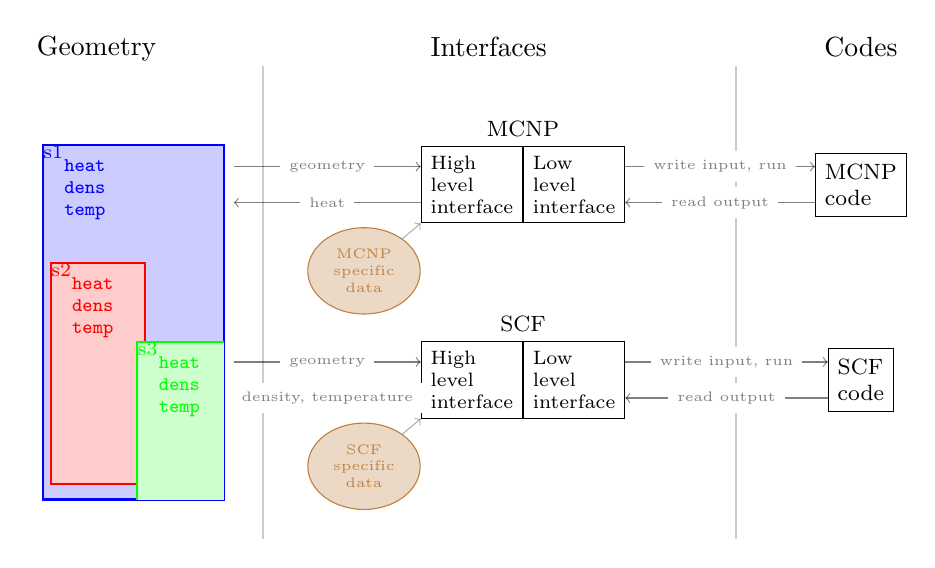
\begin{tikzpicture}
    %\draw[help lines, thin, color=blue!10] (0,0) grid (11,7);
    \tikzstyle{every node}=[font=\footnotesize]%, draw=black!10]%, draw=black, rounded corners, text centered]%, minimum height=1cm, text width=4cm]
    % Titles
    \tikzstyle{Titles}=[font=\normalsize, anchor=north west]
    \node[Titles] at (0,7) (t1) {Geometry};
    \node[Titles] at (5,7) (t2) {Interfaces};
    \node[Titles] at (10,7) (t3) {Codes};

    % vertical delimiters
    \tikzstyle{DelimiterLines}=[color=black!20, thick]
    \draw[DelimiterLines] (3, 6.5) -- +(0,-6cm);
    \draw[DelimiterLines] (9, 6.5) -- +(0,-6cm);

    % model example
    \coordinate (m1) at (0.2, 1);
    \coordinate (m2) at (2.5, 5.5);
    \coordinate (m3) at (0.3, 1.2);
    \coordinate (m4) at (1.5, 4.0);
    \coordinate (m5) at (1.4, -1);
    \coordinate (m6) at (2.7, 3.0);
    \node[opacity=0., fit=(m1) (m2)] (model) {};
    \begin{scope}% scope here while clipping.
        \path[clip] 
            [preaction = {draw=blue,thick, fill=blue!20}]
            (m1) rectangle (m2);
        \path[thick, fill=red!20,   draw=red]   (m3) rectangle (m4);
        \path[thick, fill=green!20, draw=green] (m5) rectangle (m6);
    \end{scope}
    
    \tikzstyle{SolidLabels}=[align=right,font=\scriptsize, opacity=0., text opacity=1., inner sep=0., anchor=north west]
    \tikzstyle{MeshLabels}=[SolidLabels,font=\scriptsize\tt]
    \node[SolidLabels, text=blue] at (m1 |- m2) (s1) {s1};
    \node[SolidLabels, text=red]   at (m3 |- m4) (s2) {s2};
    \node[SolidLabels, text=green] at (m5 |- m6) (s3) {s3};

    \node[MeshLabels,  text=blue,  below right=0mm of s1] (m1) {heat\\dens\\temp};
    \node[MeshLabels,  text=red,   below right=0mm of s2] (m2) {heat\\dens\\temp};
    \node[MeshLabels,  text=green, below right=0mm of s3] (m3) {heat\\dens\\temp};

    % % interfaces
    \tikzstyle{Interfaces}=[draw=black,rectangle split, rectangle split parts=2, rectangle split horizontal=true, minimum height=0.8cm, align=left,font=\scriptsize]
    \tikzstyle{SpecData}=[color=brown, draw, fill, ellipse, align=center, font=\tiny, opacity=1, fill opacity=0.3, text opacity=1.]

    \node[Interfaces, anchor=west, label=above:MCNP] at (5, 5) (mi) {High\\level\\interface \nodepart{second} Low\\level\\interface};
    \node[SpecData, below left=3mm of mi] (msd) {MCNP\\specific\\data};

    \node[Interfaces, below=15mm of mi, label=above:SCF] (si) {High\\level\\interface \nodepart{second} Low\\level\\interface};
    \node[SpecData, below left=3mm of si] (ssd) {SCF\\specific\\data};



    % codes
    \tikzstyle{Codes}=[draw=black, minimum height=0.8cm, align=left]
    \node[Codes, align=left] at (t3 |- mi) (mcnp) {MCNP\\code};
    \node[Codes, align=left] at (t3 |- si) (scf)  {SCF\\code};


    %% connections
    \tikzstyle{ConnectionNodes}=[font=\tiny, fill=white, fill opacity=1., text opacity=0.5, align=center]
    \tikzstyle{ConnectionLines}=[opacity=0.5]

    % model -- MCNP interface
    \draw[ConnectionLines, ->] (model.east |- mi.170) -- node[ConnectionNodes] {geometry} (mi.170);
    \draw[ConnectionLines, <-] (model.east |- mi.190) -- node[ConnectionNodes] {heat}     (mi.190);

    % MCNP interface -- MCNP
    \draw[ConnectionLines, ->] (mi.10)  -- node[ConnectionNodes] {write input, run} (mcnp.west |- mi.10);
    \draw[ConnectionLines, <-] (mi.-10) -- node[ConnectionNodes] {read output}      (mcnp.west |- mi.-10);

    % model -- SCF interface
    \draw[ConnectionLines, ->] (model.east |- si.170) -- node[ConnectionNodes] {geometry}             (si.170);
    \draw[ConnectionLines, <-] (model.east |- si.190) -- node[ConnectionNodes] {density, temperature} (si.190);

    % SCF interface -- SCF
    \draw[ConnectionLines, ->] (si.10)  -- node[ConnectionNodes] {write input, run} (scf.west |- si.10);
    \draw[ConnectionLines, <-] (si.-10) -- node[ConnectionNodes] {read output}      (scf.west |- si.-10);

    % code specific data
    \draw[ConnectionLines, ->, opacity=0.3] (msd) -- (mi.south west);
    \draw[ConnectionLines, ->, opacity=0.3] (ssd) -- (si.south west);



\end{tikzpicture}

\end{frame}


\begin{frame}\frametitle{Concept}
    \begin{block}{Classes provided by PIRS fall into three catogories}
        \begin{itemize}
            \item To describe calculation geometry:
                  Solids (Cylinder, Box) can be inserted into each other and
                  positioned with respect to container.

            \item Low-level interfaces:
                \begin{itemize}
                    \item Assure correct syntax of input file, 
                    \item "Know" command line parameters of the code, 
                    \item provide functions to read output. 
                \end{itemize}

            \item High-level interfaces:
                \begin{itemize}
                    \item Conversion: geometry $\Longleftrightarrow$ low-level interfaces,
                    \item Interface to specify code-specific parameters
                \end{itemize}
        \end{itemize}
    \end{block}
\end{frame}


%%%%%%%%%%%%%%%%%%%%%%%%%%%%%%%%%%%%%%%%%%%%%%%%%%%%%%%%%%%%%%%%%%%%%%%%%%%%%%%%%%%%%%%%%%%%%%%%%%%%%
\section{Example: fuel pin neutronics model}

\newcommand{\exModel}{Example: simplified neutronics model of fuel pin}
\begin{frame}[fragile]
    \frametitle{\exModel}

    Geometry definition:
    \inputminted[frame=single,fontfamily=tt,fontsize=\footnotesize]{python}{geom.py}

\end{frame}

\begin{frame}[fragile]
    \frametitle{\exModel}

    MCNP interface:

    \begin{columns}
        \column{0.45\textwidth}
            \inputminted[frame=single,fontfamily=tt,fontsize=\footnotesize,firstline=3,lastline=17]{python}{mc_int.py}
        \column{0.45\textwidth}
            \inputminted[frame=single,fontfamily=tt,fontsize=\footnotesize,firstline=17]{python}{mc_int.py}
    \end{columns}

\end{frame}

\begin{frame}[fragile,plain]
    \frametitle{\exModel}
    \begin{columns}
        \column{0.45\textwidth}
            {\tiny Generated MCNP input file}
            \inputminted[frame=single,fontfamily=tt,fontsize=\tiny,firstline=3,lastline=33]{rst}{mcnp0/i_}
        \column{0.45\textwidth}
            \inputminted[frame=single,fontfamily=tt,fontsize=\tiny,firstline=34]{rst}{mcnp0/i_}
    \end{columns}
\end{frame}

\begin{frame}[fragile]
    \frametitle{\exModel}

    {\small Geometry plot generated with MCNP}
    \includegraphics[width=0.7\textwidth]{mcnp0/i__p02.pdf}
\end{frame}


%%%%%%%%%%%%%%%%%%%%%%%%%%%%%%%%%%%%%%%%%%%%%%%%%%%%%%%%%%%%%%%%%%%%%%%%%%%%%%%%%%%%%%%%%%%%%%%%%%%%%
\section{Example: results of MCNP-SCF coupled calculations}

\newcommand{\exResult}{Example: results for coupled MCNP-SCF calculations}
\begin{frame}\frametitle{\exResult}

    Coupled MCNP -- SCF calculations, organized with PIRS
    \begin{itemize}
        \item Model: PWR assembly 17x17,
        \item moderator channels,
        \item two different types of fuel pins,
        \item boron in coolant,
        \item Coolant-centered subchannels,
        \item non-uniform axial mesh,
        \item Calculations conducted on a linux desktop
        \item relaxation scheme for power axial distribution with varying relaxation parameter and increasing statistical precision

    \end{itemize}

\end{frame}

\begin{frame}\frametitle{\exResult}

    Horizontal cross-section of MCNP model:
    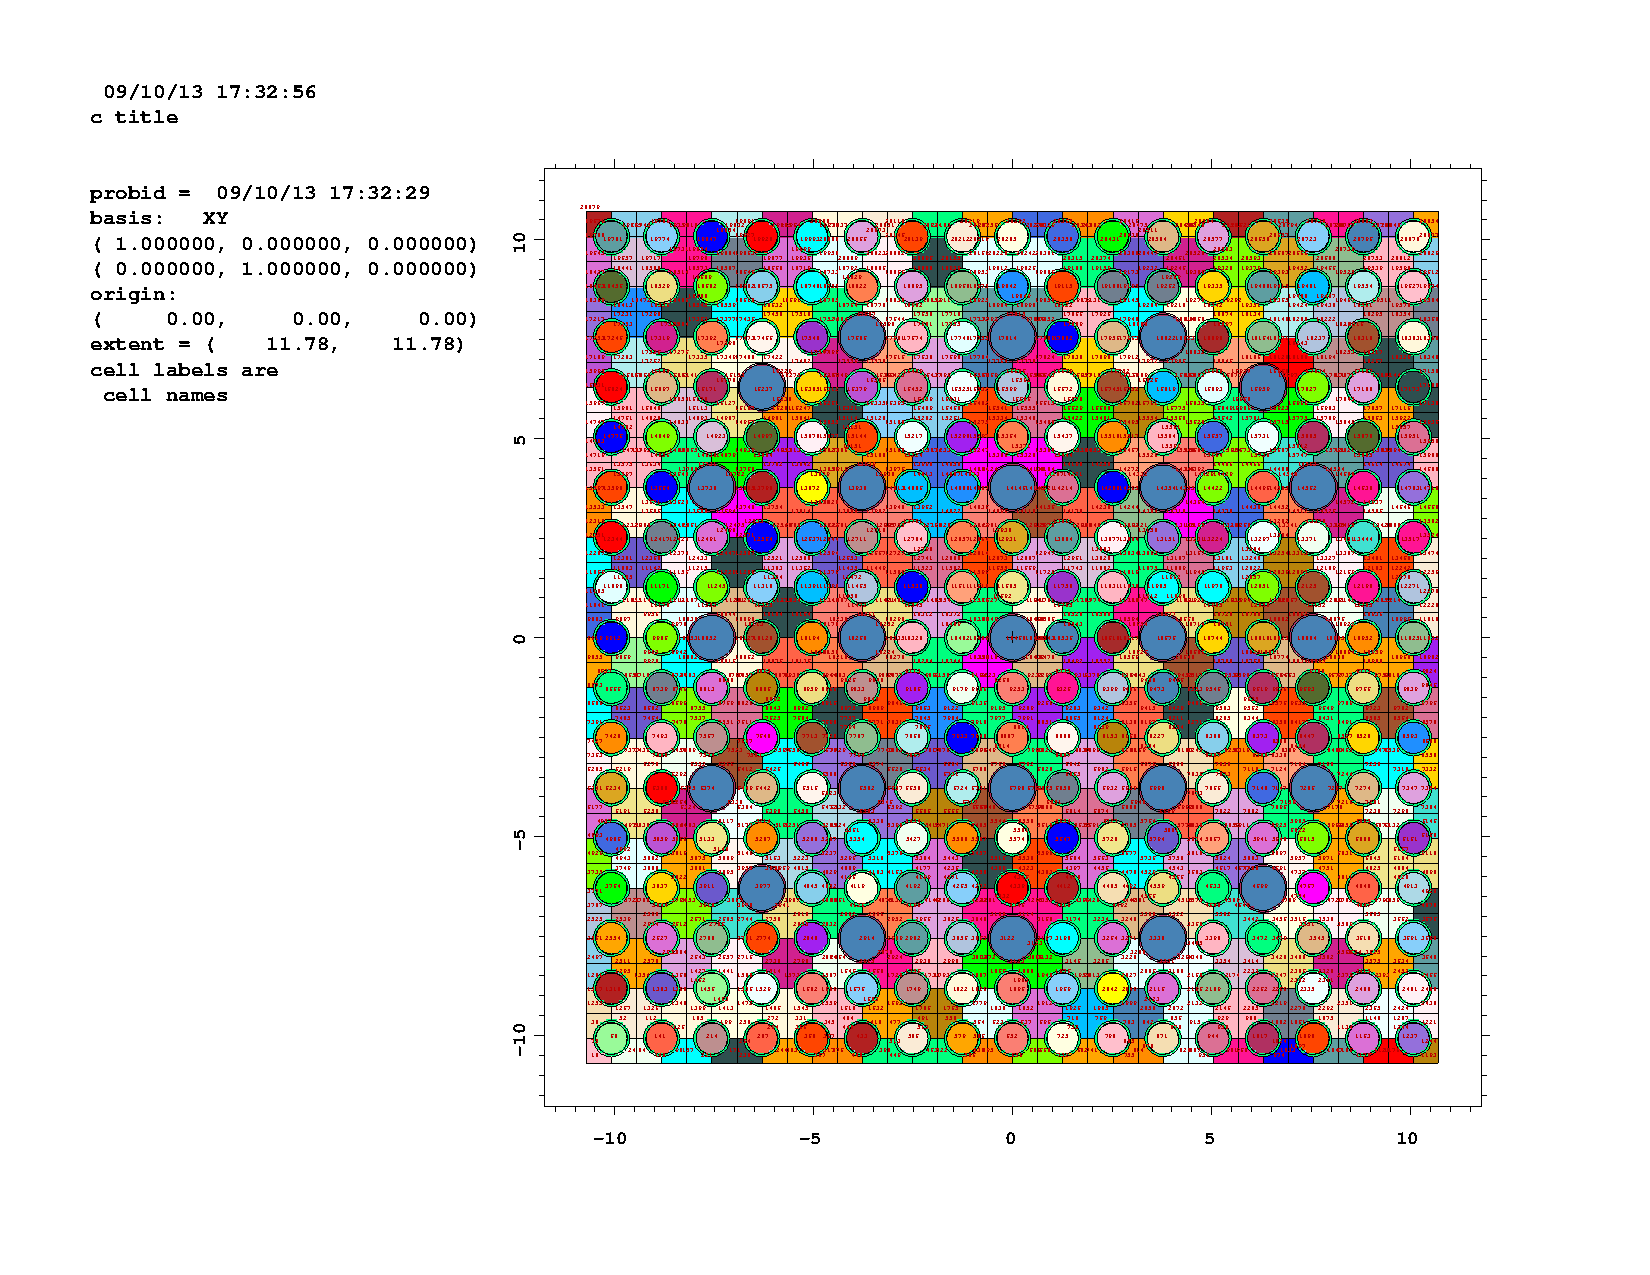
\includegraphics[width=0.7\textwidth]{pics/i__p01.pdf}

\end{frame}
\begin{frame}\frametitle{\exResult}

    Vertical cross-section of MCNP model:
    \includegraphics[width=0.7\textwidth]{pics/i__p02.pdf}

\end{frame}
\begin{frame}\frametitle{\exResult}

    Behaviour of  $k_{eff}$ with N--TH iterations 
    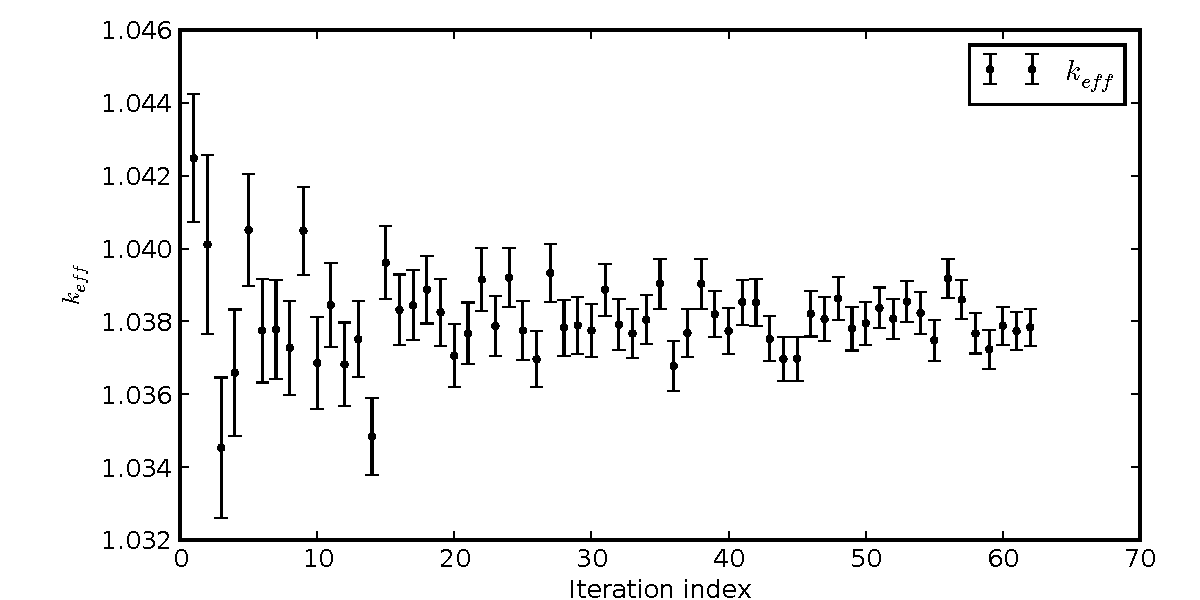
\includegraphics[width=0.8\textwidth]{pics/b_iteration_062_keff.pdf}
\end{frame}

\begin{frame}\frametitle{\exResult}
    Axial distribution of heat deposition in one fuel pin

    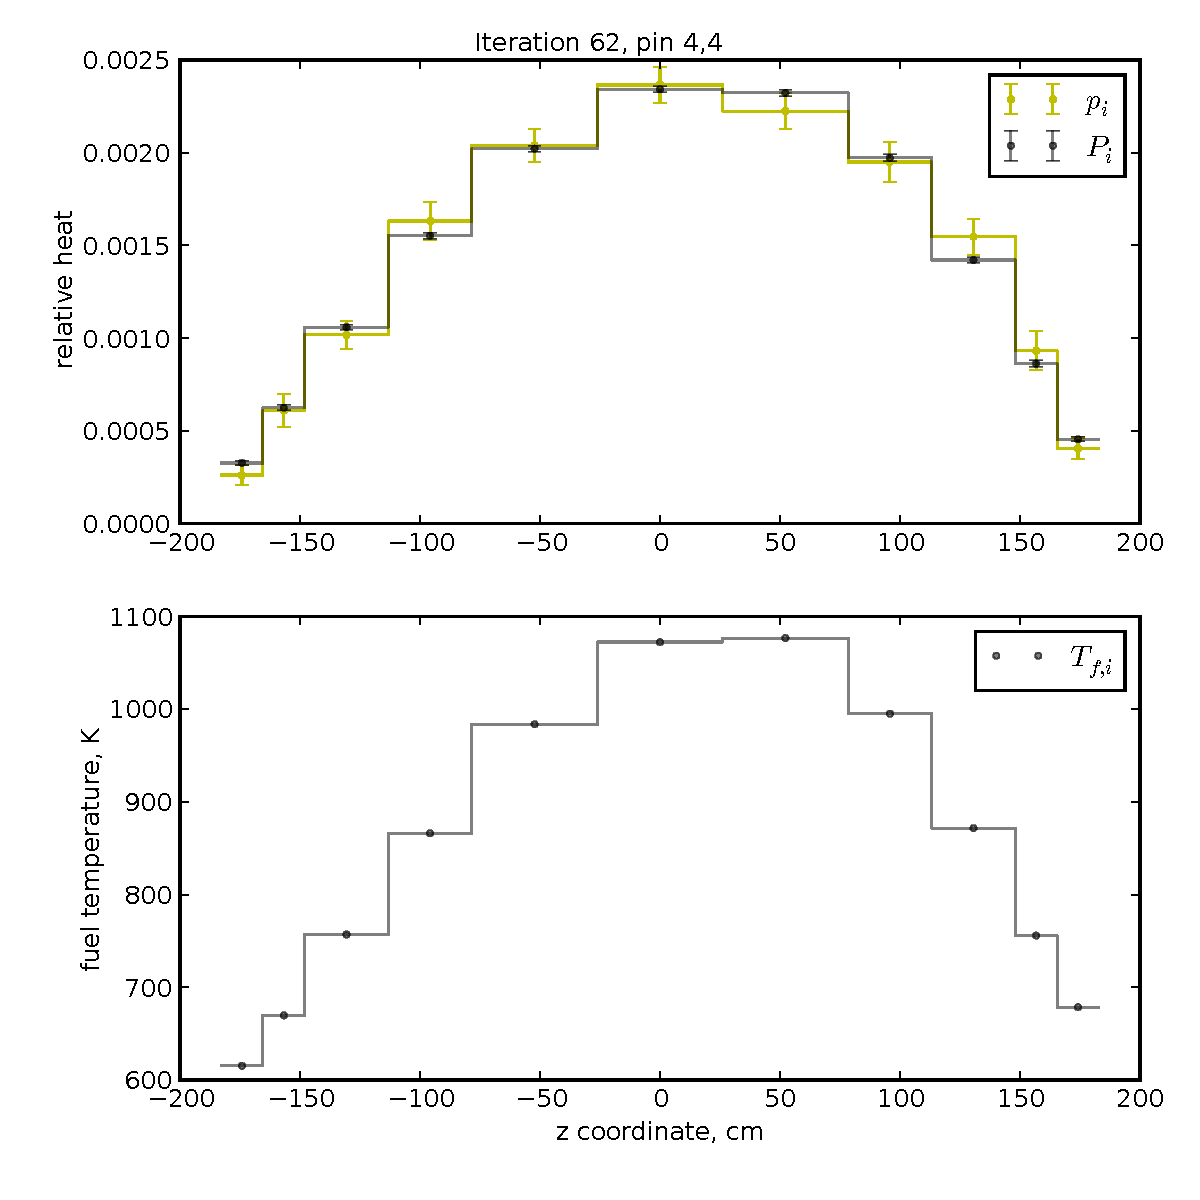
\includegraphics[trim=0 300 0 0,clip=true,width=0.8\textwidth]{pics/b_iteration_062_4_4.pdf}
\end{frame}

\begin{frame}\frametitle{\exResult}
    Axial distribution of fuel temperature in the same pin

    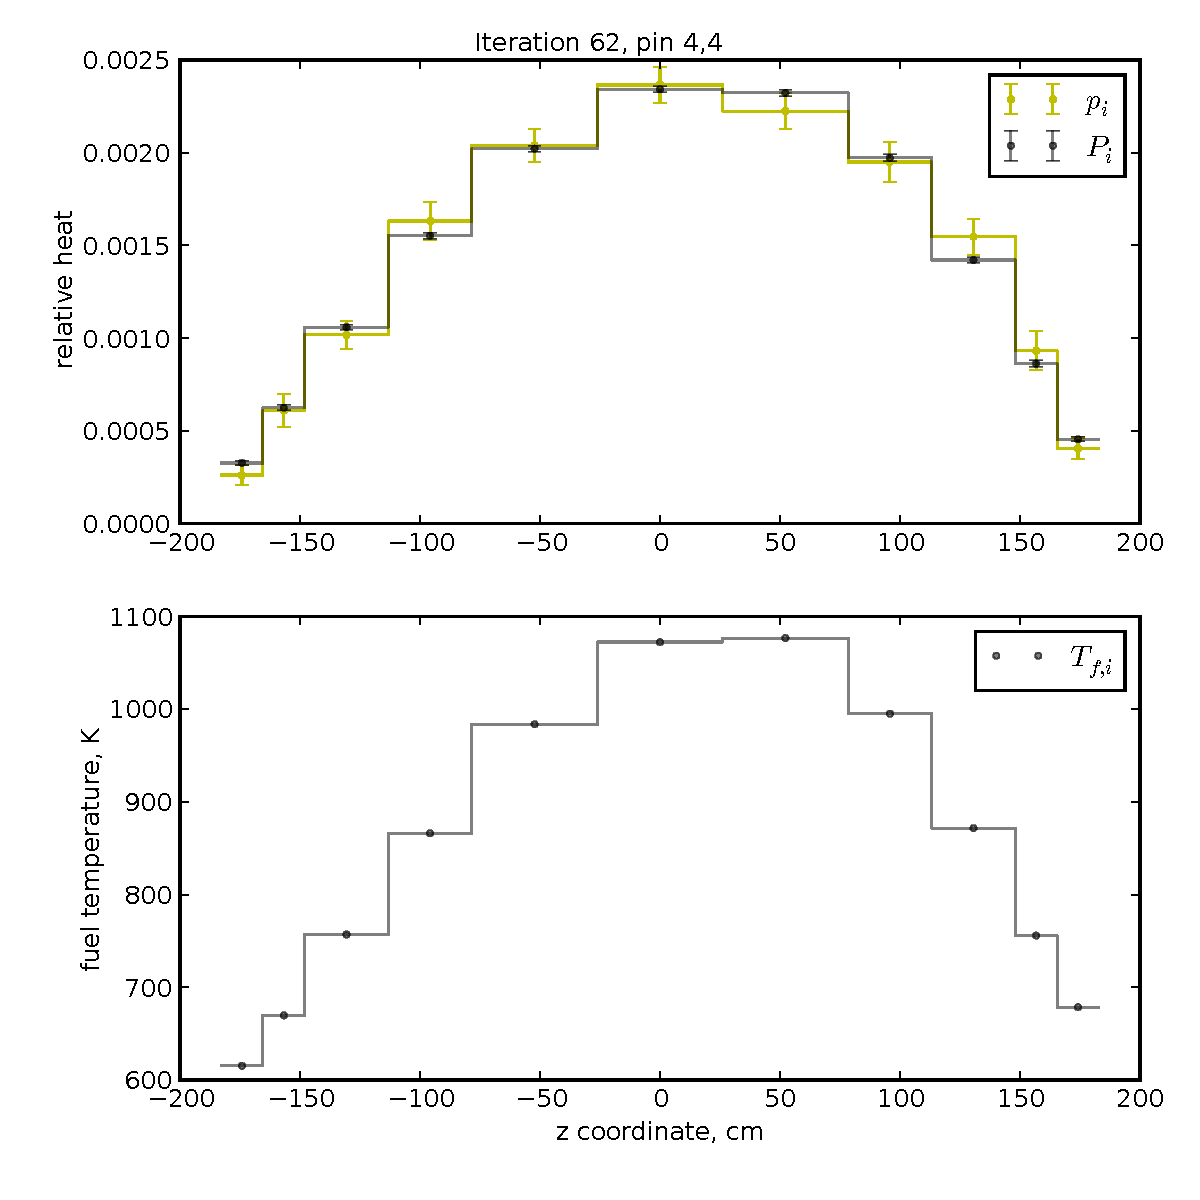
\includegraphics[trim=0 0 0 280,clip=true,width=0.8\textwidth]{pics/b_iteration_062_4_4.pdf}
\end{frame}

\begin{frame}\frametitle{\exResult}
    Temperature map

    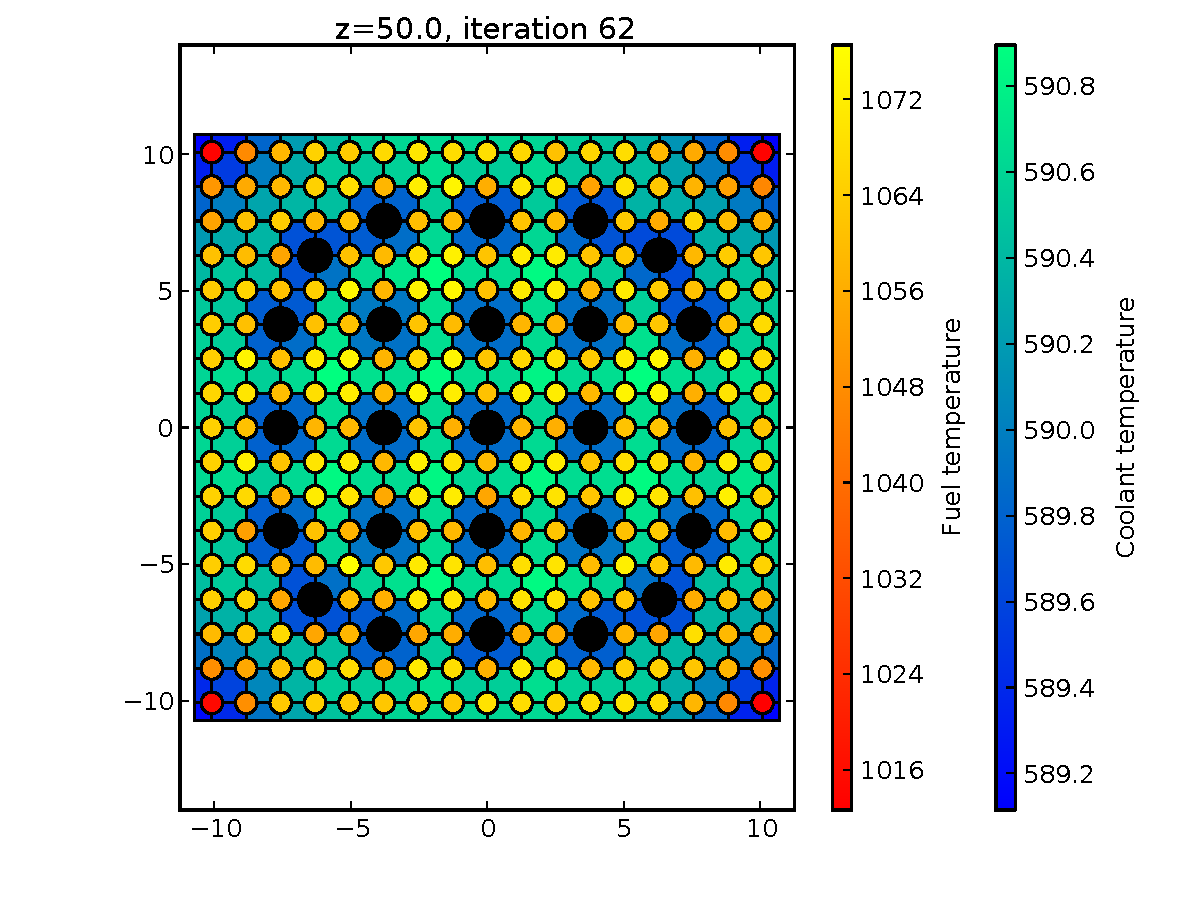
\includegraphics[width=0.7\textwidth]{pics/b_iteration_062_temp50_0.pdf}
\end{frame}

%%%%%%%%%%%%%%%%%%%%%%%%%%%%%%%%%%%%%%%%%%%%%%%%%%%%%%%%%%%%%%%%%%%%%%%%%%%%%%%%%%%%%%%%%%%%%%%%%%%%%
\section{Current development status}
\begin{frame}\frametitle{Current development status}
    Governed by HPMC project: Monte-Carlo neutronics and sub-channel TH modelling of PWR assembly and core.

    
    \begin{columns}
    \column{0.47\textwidth}
    \begin{block}{Interface to MCNP}
        \begin{itemize}
            \item handles any geometry represented by boxes and cylinders
            \item Repeated structure can be modelled as lattice 
            \item Description of materials
                \begin{itemize}
                    \item Convenient definition of composition
                    \item Automatic choice of suffixes and interpolation of XS
                \end{itemize}
            \item Reads meshtal
        \end{itemize}
    \end{block}

    \column{0.47\textwidth}
    \begin{block}{Means to set up geometry} 
        \begin{itemize}
            \item Cylinder: vertical cylinder of finite height
            \item Box: rectangular parallelepiped with facets perpendicular to axes
            \item meshes to represent temperature, density and heat axial profiles
        \end{itemize}
    \end{block}
    \begin{block}{Interface to SCF}
        \begin{itemize}
            \item Only for PWR-like geometries
            \item Reads output.txt
        \end{itemize}
    \end{block}
    \end{columns}

\end{frame}


%%%%%%%%%%%%%%%%%%%%%%%%%%%%%%%%%%%%%%%%%%%%%%%%%%%%%%%%%%%%%%%%%%%%%%%%%%%%%%%%%%%%%%%%%%%%%%%%%%%%%
\section{Ongoing work}
\begin{frame}\frametitle{Ongoing work}

    \begin{block}{Current}
        \begin{itemize}
            \item calculation of a minicore $\rightarrow$ optimization of MCNP and SCF interfaces
        \end{itemize}
    \end{block}

    \begin{block}{Plans}
        \begin{itemize}
            \item Interface to SERPENT-2
            \item New interface to SCF
            \item update Documentation, open source
            \item Geometry plotter
            \item interfaces to other codes?
        \end{itemize}
    \end{block}

\end{frame}


\end{document}
